% Chapter 2: Seminar - ARMA Models
% Harvard-quality academic presentation
% Bachelor program, Bucharest University of Economic Studies

\documentclass[9pt, aspectratio=169, t]{beamer}

% Ensure content fits on slides
\setbeamersize{text margin left=8mm, text margin right=8mm}

%=============================================================================
% THEME AND STYLE CONFIGURATION
%=============================================================================
\usetheme{default}
% Using default theme for clean header/footer control

% Color Palette (matching Redispatch PDF)
\definecolor{MainBlue}{RGB}{26, 58, 110}
\definecolor{AccentBlue}{RGB}{26, 58, 110}
\definecolor{IDAred}{RGB}{205, 0, 0}
\definecolor{DarkGray}{RGB}{51, 51, 51}
\definecolor{MediumGray}{RGB}{128, 128, 128}
\definecolor{LightGray}{RGB}{248, 248, 248}
\definecolor{VeryLightGray}{RGB}{235, 235, 235}
\definecolor{KeynoteGray}{RGB}{218, 218, 218}
\definecolor{SectionGray}{RGB}{120, 120, 120}
\definecolor{FooterGray}{RGB}{100, 100, 100}
\definecolor{Crimson}{RGB}{220, 53, 69}
\definecolor{Forest}{RGB}{46, 125, 50}
\definecolor{Amber}{RGB}{181, 133, 63}
\definecolor{Orange}{RGB}{230, 126, 34}
\definecolor{Purple}{RGB}{142, 68, 173}

% Gradient background (exact Keynote 315° gradient: white to RGB 218,218,218)
\setbeamertemplate{background}{%
    \begin{tikzpicture}[remember picture, overlay]
        \shade[shading=axis, shading angle=315,
        top color=white, bottom color=KeynoteGray]
        (current page.south west) rectangle (current page.north east);
    \end{tikzpicture}%
}
% Fallback solid color for compatibility
\setbeamercolor{background canvas}{bg=}

\setbeamercolor{palette primary}{bg=MainBlue, fg=white}
\setbeamercolor{palette secondary}{bg=MainBlue!85, fg=white}
\setbeamercolor{palette tertiary}{bg=MainBlue!70, fg=white}
\setbeamercolor{structure}{fg=MainBlue}
\setbeamercolor{title}{fg=IDAred}
\setbeamercolor{frametitle}{fg=IDAred, bg=}
\setbeamercolor{block title}{bg=MainBlue, fg=white}
\setbeamercolor{block body}{bg=VeryLightGray, fg=DarkGray}
\setbeamercolor{block title alerted}{bg=Crimson, fg=white}
\setbeamercolor{block body alerted}{bg=Crimson!8, fg=DarkGray}
\setbeamercolor{block title example}{bg=Forest, fg=white}
\setbeamercolor{block body example}{bg=Forest!8, fg=DarkGray}
\setbeamercolor{item}{fg=MainBlue}

% Footer colors (override Madrid theme blue)
\setbeamercolor{author in head/foot}{fg=FooterGray, bg=}
\setbeamercolor{title in head/foot}{fg=FooterGray, bg=}
\setbeamercolor{date in head/foot}{fg=FooterGray, bg=}
\setbeamercolor{section in head/foot}{fg=FooterGray, bg=}
\setbeamercolor{subsection in head/foot}{fg=FooterGray, bg=}

% Bullet styles (apply everywhere including blocks)
\setbeamertemplate{itemize item}{\color{MainBlue}$\boxdot$}
\setbeamertemplate{itemize subitem}{\color{MainBlue}$\blacktriangleright$}
\setbeamertemplate{itemize subsubitem}{\color{MainBlue}\tiny$\bullet$}
\setbeamertemplate{itemize/enumerate body begin}{\normalsize}
\setbeamertemplate{itemize/enumerate subbody begin}{\normalsize}

% Item spacing - compact style
\setlength{\leftmargini}{10pt}       % Level 1: minimal indent
\setlength{\leftmarginii}{10pt}      % Level 2: minimal additional indent
% Compact list spacing (zero extra space before/after lists in blocks)
\makeatletter
\def\@listi{\leftmargin\leftmargini \topsep 0pt \parsep 0pt \itemsep 0pt}
\def\@listii{\leftmargin\leftmarginii \topsep 0pt \parsep 0pt \itemsep 0pt}
\makeatother

\setbeamertemplate{navigation symbols}{}

%=============================================================================
% CUSTOM HEADLINE
%=============================================================================
\setbeamertemplate{headline}{%
    \vskip10pt%
    \hbox to \paperwidth{%
        \hskip0.5cm%
        {\small\color{FooterGray}\renewcommand{\hyperlink}[2]{##2}\insertsectionhead}%
        \hfill%
        \textcolor{FooterGray}{\small\insertframenumber}%
        \hskip0.5cm%
    }%
    \vskip4pt%
    {\color{FooterGray}\hrule height 0.4pt}%
}

%=============================================================================
% CUSTOM FOOTER
%=============================================================================
\usepackage{fontawesome5}

\setbeamertemplate{footline}{%
    {\color{FooterGray}\hrule height 0.4pt}%
    \vskip4pt%
    \hbox to \paperwidth{%
        \hskip0.5cm%
        \textcolor{FooterGray}{\small Time Series Analysis and Forecasting}%
        \hfill%
        \raisebox{-0.1em}{%
            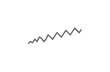
\begin{tikzpicture}[x=0.08em, y=0.08em, line width=0.4pt]
                \draw[FooterGray] (0,3) -- (1,4) -- (2,3.5) -- (3,5) -- (4,4) -- (5,6) -- (6,5.5) -- (7,4) -- (8,5) -- (9,7) -- (10,6) -- (11,5) -- (12,6.5) -- (13,8) -- (14,7) -- (15,6) -- (16,7.5) -- (17,9) -- (18,8) -- (19,7) -- (20,8.5) -- (21,10) -- (22,9) -- (23,8) -- (24,9.5);
            \end{tikzpicture}%
        }%
        \hskip0.5cm%
    }%
    \vskip6pt%
}

%=============================================================================
% PACKAGES
%=============================================================================
\usepackage[utf8]{inputenc}
\usepackage[T1]{fontenc}
\usepackage[english]{babel}
\usepackage{amsmath, amssymb, amsthm}
\usepackage{mathtools}
\usepackage{bm}
\usepackage{tikz}
\usetikzlibrary{arrows.meta, positioning, shapes, calc, decorations.pathreplacing, shadings}
\usepackage{booktabs}
\usepackage{multirow}
\usepackage{array}
\usepackage{graphicx}
\usepackage{hyperref}
\usepackage{colortbl}
\hypersetup{colorlinks=true, linkcolor=MainBlue, urlcolor=MainBlue}
\graphicspath{{../../logos/}{../../charts/}}
\hfuzz=2pt  % Suppress tiny overfull warnings (<2pt)
\vfuzz=2pt  % Suppress tiny vertical overfull warnings (<2pt)

%=============================================================================
% QUANTLET COMMAND
%=============================================================================
\newcommand{\quantlet}[2]{%
    \hfill\href{#2}{%
        \raisebox{-0.15em}{\includegraphics[height=0.7em]{ql_logo.png}}%
        \textcolor{MainBlue}{\tiny\ #1}%
    }%
}

%=============================================================================
% CUSTOM COMMANDS
%=============================================================================
\newcommand{\E}{\mathbb{E}}
\newcommand{\Var}{\text{Var}}
\newcommand{\Cov}{\text{Cov}}
\newcommand{\Corr}{\text{Corr}}
\newcommand{\R}{\mathbb{R}}
\newcommand{\RMSE}{\text{RMSE}}
\newcommand{\MAE}{\text{MAE}}
\newcommand{\MAPE}{\text{MAPE}}

% Quiz styling
\newcommand{\correct}{\textcolor{Forest}{\checkmark}}
\newcommand{\incorrect}{\textcolor{Crimson}{\texttimes}}

%=============================================================================
% CUSTOM TITLE PAGE
%=============================================================================
\defbeamertemplate*{title page}{hybrid}[1][]
{
    \vspace{0.2cm}
    % Logos row - top header (with clickable links)
    \begin{center}
        \href{https://www.ase.ro}{\includegraphics[height=1.0cm]{ase_logo.png}}\hspace{0.3cm}%
        \href{https://theida.net}{\includegraphics[height=1.0cm]{ida_logo.png}}\hspace{0.3cm}%
        \href{https://blockchain-research-center.com}{\includegraphics[height=1.0cm]{brc_logo.png}}\hspace{0.3cm}%
        \href{https://www.ai4efin.ase.ro}{\includegraphics[height=1.0cm]{ai4efin_logo.png}}\hspace{0.3cm}%
        \href{https://ipe.ro/new}{\includegraphics[height=1.0cm]{acad_logo.png}}\hspace{0.3cm}%
        \href{https://www.digital-finance-msca.com}{\includegraphics[height=1.0cm]{msca_logo.png}}%
    \end{center}

    \vspace{0.6cm}

    % Main title with Q logos on sides (with clickable links)
    \begin{center}
        \begin{minipage}{0.1\textwidth}
            \centering
            \href{https://quantlet.com}{\includegraphics[height=1.1cm]{ql_logo.png}}
        \end{minipage}%
        \begin{minipage}{0.78\textwidth}
            \centering
            {\LARGE\bfseries\usebeamercolor[fg]{title}\inserttitle}

            \vspace{0.3cm}

            {\usebeamerfont{subtitle}\usebeamercolor[fg]{title}\insertsubtitle}
        \end{minipage}%
        \begin{minipage}{0.1\textwidth}
            \centering
            \href{https://quantinar.com}{\includegraphics[height=1.1cm]{qr_logo.png}}
        \end{minipage}
    \end{center}

    \vspace{0.6cm}

    % Authors (left aligned)
    \hspace{0.5cm}{\usebeamerfont{author}\insertauthor}

    \vspace{0.3cm}

    % Institute/Affiliations (left aligned)
    \hspace{0.5cm}\begin{minipage}[t]{0.9\textwidth}
        \raggedright\small\insertinstitute
    \end{minipage}
}

%=============================================================================
% TITLE INFORMATION
%=============================================================================
\title[Time Series Analysis]{Time Series Analysis and Forecasting}
\subtitle{Seminar 2: ARMA Models}
\author[D.T. Pele]{Daniel Traian PELE}
\institute{Academia de Studii Economice din Bucure\c{s}ti\\
IDA Institute Digital Assets\\
Blockchain Research Center\\
AI4EFin Artificial Intelligence for Energy Finance\\
Academia Rom\^{a}n\u{a}, Institutul de Prognoz\u{a} Economic\u{a}\\
MSCA Digital Finance}
\date{}

\begin{document}

% Title page (no header/footer)
{
\setbeamertemplate{headline}{}
\setbeamertemplate{footline}{}
\begin{frame}
    \titlepage
\end{frame}
}

%=============================================================================
% SEMINAR OUTLINE
%=============================================================================
\section{Overview}

\begin{frame}{Seminar Outline}
    \textbf{\large Today's Activities:}

    \vspace{0.4cm}

    \begin{enumerate}
        \item[\textcolor{MainBlue}{\textbf{1.}}] \textbf{Review Quiz} --- Checking understanding of ARMA concepts
        \vspace{0.15cm}
        \item[\textcolor{MainBlue}{\textbf{2.}}] \textbf{True/False Questions} --- Conceptual checks
        \vspace{0.15cm}
        \item[\textcolor{MainBlue}{\textbf{3.}}] \textbf{Practice Problems} --- Practice with AR/MA
        \vspace{0.15cm}
        \item[\textcolor{MainBlue}{\textbf{4.}}] \textbf{Worked Examples} --- Fitting and diagnostics
        \vspace{0.15cm}
        \item[\textcolor{MainBlue}{\textbf{5.}}] \textbf{Discussion Topics} --- Practical applications
        \vspace{0.15cm}
        \item[\textcolor{MainBlue}{\textbf{6.}}] \textbf{AI-Assisted Exercises} --- Human vs.\ AI modeling
    \end{enumerate}
\end{frame}

%=============================================================================
% PART 1: REVIEW QUIZ
%=============================================================================
\section{Review Quiz}

\begin{frame}{Quiz 1: Lag Operator}
    \begin{alertblock}{Question}
        What is the result of applying $(1-L)^2$ to $X_t$?
    \end{alertblock}

    \vspace{0.5cm}
    \setlength{\leftmargini}{2cm}
    \begin{enumerate}[A.]
        \item $X_t - X_{t-1}$
        \item $X_t - 2X_{t-1} + X_{t-2}$
        \item $X_t + X_{t-1} + X_{t-2}$
        \item $X_t - X_{t-2}$
    \end{enumerate}
\end{frame}

\begin{frame}{Quiz 1: Answer}
    \vspace{0.3cm}
    \begin{center}
        \includegraphics[width=0.75\textwidth, height=0.38\textheight, keepaspectratio]{lag_operator.pdf}
    \end{center}
    \vspace{-0.1cm}

    \begin{exampleblock}{Answer: B}
        $X_t - 2X_{t-1} + X_{t-2}$
    \end{exampleblock}

    \textbf{Explanation:}
    $(1-L)^2 X_t = (1 - 2L + L^2)X_t = X_t - 2X_{t-1} + X_{t-2}$ --- the \textbf{second difference} of $X_t$.

    \quantlet{TSA\_ch2\_lag\_operator}{https://github.com/QuantLet/TSA/tree/main/TSA_ch2/TSA_ch2_lag_operator}
\end{frame}

\begin{frame}{Quiz 2: AR(1) Stationarity}
    \begin{alertblock}{Question}
        For which value of $\phi$ is the AR(1) process $X_t = 0.5 + \phi X_{t-1} + \varepsilon_t$ stationary?
    \end{alertblock}

    \vspace{0.5cm}
    \setlength{\leftmargini}{2cm}
    \begin{enumerate}[A.]
        \item $\phi = 1.2$
        \item $\phi = 1.0$
        \item $\phi = -0.8$
        \item $\phi = -1.5$
    \end{enumerate}
\end{frame}

\begin{frame}{Quiz 2: Answer}
    \vspace{0.3cm}
    \begin{center}
        \includegraphics[width=0.75\textwidth, height=0.38\textheight, keepaspectratio]{ch2_def_ar1.pdf}
    \end{center}
    \vspace{-0.1cm}

    \begin{exampleblock}{Answer: C}
        $\phi = -0.8$ (Stationary)
    \end{exampleblock}

    \textbf{AR(1) stationarity condition:} $|\phi| < 1$. Checking each option:
    \begin{itemize}
        \item A: $|1.2| = 1.2 > 1$ \incorrect \quad B: $|1.0| = 1$ (unit root) \incorrect \quad C: $|-0.8| = 0.8 < 1$ \correct \quad D: $|-1.5| = 1.5 > 1$ \incorrect
    \end{itemize}

    \quantlet{TSA\_ch2\_ar1}{https://github.com/QuantLet/TSA/tree/main/TSA_ch2/TSA_ch2_ar1}
\end{frame}

\begin{frame}{Quiz 3: ACF Pattern}
    \begin{alertblock}{Question}
        You observe the following ACF pattern: significant spike at lag 1, then all lags within confidence bands. PACF shows gradual decay. What model is suggested?
    \end{alertblock}

    \vspace{0.5cm}
    \setlength{\leftmargini}{2cm}
    \begin{enumerate}[A.]
        \item AR(1)
        \item MA(1)
        \item ARMA(1,1)
        \item White noise
    \end{enumerate}
\end{frame}

\begin{frame}{Quiz 3: Answer}
    \vspace{0.3cm}
    \begin{center}
        \includegraphics[width=0.75\textwidth, height=0.38\textheight, keepaspectratio]{ch2_def_ma1.pdf}
    \end{center}
    \vspace{-0.1cm}

    \begin{exampleblock}{Answer: B}
        MA(1)
    \end{exampleblock}

    \textbf{Key identification rule:}
    \begin{itemize}
        \item ACF cuts off after lag $q$ $\Rightarrow$ MA($q$); PACF cuts off after lag $p$ $\Rightarrow$ AR($p$)
    \end{itemize}

    Here: ACF cuts off at lag 1, PACF decays $\Rightarrow$ \textbf{MA(1)}

    \quantlet{TSA\_ch2\_ma1}{https://github.com/QuantLet/TSA/tree/main/TSA_ch2/TSA_ch2_ma1}
\end{frame}

\begin{frame}{Quiz 4: MA Invertibility}
    \begin{alertblock}{Question}
        For the MA(1) process $X_t = \varepsilon_t + 1.5\varepsilon_{t-1}$, is the process invertible?
    \end{alertblock}

    \vspace{0.5cm}
    \setlength{\leftmargini}{2cm}
    \begin{enumerate}[A.]
        \item Yes, because MA processes are always invertible
        \item Yes, because $1.5 > 0$
        \item No, because $|\theta| = 1.5 > 1$
        \item No, because MA processes are never invertible
    \end{enumerate}
\end{frame}

\begin{frame}{Quiz 4: Answer}
    \vspace{0.3cm}
    \begin{center}
        \includegraphics[width=0.75\textwidth, height=0.38\textheight, keepaspectratio]{ch2_def_ma1.pdf}
    \end{center}
    \vspace{-0.1cm}

    \begin{exampleblock}{Answer: C}
        Not invertible ($|\theta| = 1.5 > 1$)
    \end{exampleblock}

    \textbf{MA(1) invertibility:} Requires $|\theta| < 1$. The root of $\theta(z) = 1 + \theta z = 0$ must be outside the unit circle. Here: $z = -1/1.5 = -0.67$ is \textbf{inside}! $\Rightarrow$ \textcolor{Crimson}{\textbf{Not invertible}}

    \quantlet{TSA\_ch2\_ma1}{https://github.com/QuantLet/TSA/tree/main/TSA_ch2/TSA_ch2_ma1}
\end{frame}

\begin{frame}{Quiz 5: ARMA Representation}
    \begin{alertblock}{Question}
        The compact form $\phi(L)X_t = \theta(L)\varepsilon_t$ represents which model?
    \end{alertblock}

    \vspace{0.5cm}
    \setlength{\leftmargini}{2cm}
    \begin{enumerate}[A.]
        \item Pure AR model
        \item Pure MA model
        \item ARMA model
        \item None of the above
    \end{enumerate}
\end{frame}

\begin{frame}{Quiz 5: Answer}
    \vspace{0.3cm}
    \begin{center}
        \includegraphics[width=0.75\textwidth, height=0.38\textheight, keepaspectratio]{ch2_def_arma.pdf}
    \end{center}
    \vspace{-0.1cm}

    \begin{exampleblock}{Answer: C}
        ARMA model
    \end{exampleblock}

    \textbf{Lag polynomial notation:}
    \begin{itemize}
        \item $\phi(L) = 1 - \phi_1 L - \cdots - \phi_p L^p$; \quad $\theta(L) = 1 + \theta_1 L + \cdots + \theta_q L^q$
        \item Special cases: $\theta(L) = 1$ $\Rightarrow$ Pure AR; \quad $\phi(L) = 1$ $\Rightarrow$ Pure MA
    \end{itemize}

    \quantlet{TSA\_ch2\_arma}{https://github.com/QuantLet/TSA/tree/main/TSA_ch2/TSA_ch2_arma}
\end{frame}

\begin{frame}{Quiz 6: Information Criteria}
    \begin{alertblock}{Question}
        When comparing ARMA(1,1) and ARMA(2,1) using BIC, which statement is correct?
    \end{alertblock}

    \vspace{0.5cm}
    \setlength{\leftmargini}{2cm}
    \begin{enumerate}[A.]
        \item Lower BIC always means better forecasts
        \item BIC penalizes complexity less than AIC
        \item The model with lower BIC is preferred
        \item BIC can only compare models with the same number of parameters
    \end{enumerate}
\end{frame}

\begin{frame}{Quiz 6: Answer}
    \vspace{0.3cm}
    \begin{center}
        \includegraphics[width=0.75\textwidth, height=0.38\textheight, keepaspectratio]{ch2_acf_pacf_patterns.pdf}
    \end{center}
    \vspace{-0.1cm}

    \begin{exampleblock}{Answer: C}
        The model with lower BIC is preferred
    \end{exampleblock}

    \textbf{Information Criteria:}
    $\text{AIC} = -2\ln(\hat{L}) + 2k$; \quad $\text{BIC} = -2\ln(\hat{L}) + k\ln(n)$

    {\scriptsize $\hat{L}$ = maximum of the likelihood function, $k$ = number of parameters, $n$ = sample size}

    BIC penalizes complexity \textbf{more} than AIC (for $n > 7$) $\Rightarrow$ BIC favors simpler models.

    \quantlet{TSA\_ch2\_model\_selection}{https://github.com/QuantLet/TSA/tree/main/TSA_ch2/TSA_ch2_model_selection}
\end{frame}

\begin{frame}{Quiz 7: Ljung-Box Test}
    \begin{alertblock}{Question}
        After fitting an ARMA(2,1) model, you run the Ljung-Box test on residuals and get p-value = 0.02. What do you conclude?
    \end{alertblock}

    \vspace{0.5cm}
    \setlength{\leftmargini}{2cm}
    \begin{enumerate}[A.]
        \item The model is adequate
        \item Residuals are white noise
        \item There is significant autocorrelation in residuals
        \item The model has too many parameters
    \end{enumerate}
\end{frame}

\begin{frame}{Quiz 7: Answer}
    \vspace{0.3cm}
    \begin{center}
        \includegraphics[width=0.75\textwidth, height=0.38\textheight, keepaspectratio]{ch2_diagnostics.pdf}
    \end{center}
    \vspace{-0.1cm}

    \begin{exampleblock}{Answer: C}
        Significant autocorrelation in residuals
    \end{exampleblock}

    \textbf{Ljung-Box test:} $H_0$: Residuals are white noise; $H_1$: Autocorrelation present.

    p-value = 0.02 $<$ 0.05 $\Rightarrow$ \textcolor{Crimson}{\textbf{Reject $H_0$}}. The model is \textbf{inadequate} --- try other orders.

    \quantlet{TSA\_ch2\_diagnostics}{https://github.com/QuantLet/TSA/tree/main/TSA_ch2/TSA_ch2_diagnostics}
\end{frame}

\begin{frame}{Quiz 8: Forecasting}
    \begin{alertblock}{Question}
        For an AR(1) model with $\phi = 0.6$ and mean $\mu = 10$, what happens to forecasts as horizon $h \to \infty$?
    \end{alertblock}

    \vspace{0.5cm}
    \setlength{\leftmargini}{2cm}
    \begin{enumerate}[A.]
        \item Forecasts grow without bound
        \item Forecasts converge to 0
        \item Forecasts converge to $\mu = 10$
        \item Forecasts oscillate forever
    \end{enumerate}
\end{frame}

\begin{frame}{Quiz 8: Answer}
    \vspace{0.3cm}
    \begin{center}
        \includegraphics[width=0.75\textwidth, height=0.38\textheight, keepaspectratio]{ch2_ar1_forecast.pdf}
    \end{center}
    \vspace{-0.1cm}

    \begin{exampleblock}{Answer: C}
        Forecasts converge to $\mu = 10$
    \end{exampleblock}

    \textbf{AR(1) forecast formula:} $\hat{X}_{n+h|n} = \mu + \phi^h(X_n - \mu)$

    Since $|\phi| = 0.6 < 1$: $\lim_{h \to \infty} \phi^h = 0$ $\Rightarrow$ Forecasts converge to $\mu$. \textbf{Mean reversion!}

    \quantlet{TSA\_ch2\_forecasting}{https://github.com/QuantLet/TSA/tree/main/TSA_ch2/TSA_ch2_forecasting}
\end{frame}

\begin{frame}{Quiz 9: AR(2) Roots}
    \begin{alertblock}{Question}
        An AR(2) process has characteristic roots $z_1 = 0.8$ and $z_2 = -0.5$. Is it stationary?
    \end{alertblock}

    \vspace{0.5cm}
    \setlength{\leftmargini}{2cm}
    \begin{enumerate}[A.]
        \item Yes, because both roots are inside the unit circle
        \item No, because one root is negative
        \item No, because roots must be outside the unit circle
        \item Cannot determine without more information
    \end{enumerate}
\end{frame}

\begin{frame}{Quiz 9: Answer}
    \vspace{0.3cm}
    \begin{center}
        \includegraphics[width=0.75\textwidth, height=0.38\textheight, keepaspectratio]{ch2_ar2_stationarity.pdf}
    \end{center}
    \vspace{-0.1cm}

    \begin{exampleblock}{Answer: C}
        Roots must be outside the unit circle
    \end{exampleblock}

    \textbf{Stationarity condition:} The roots of $\phi(z) = 0$ must be \textbf{outside} the unit circle ($|z| > 1$).

    Here: $|z_1| = 0.8 < 1$ \incorrect; \quad $|z_2| = 0.5 < 1$ \incorrect. Both inside $\Rightarrow$ \textcolor{Crimson}{\textbf{Non-stationary}}

    \quantlet{TSA\_ch2\_ar2}{https://github.com/QuantLet/TSA/tree/main/TSA_ch2/TSA_ch2_ar2}
\end{frame}

\begin{frame}{Quiz 10: MA(q) Properties}
    \begin{alertblock}{Question}
        For an MA(2) process, the ACF:
    \end{alertblock}

    \vspace{0.5cm}
    \setlength{\leftmargini}{2cm}
    \begin{enumerate}[A.]
        \item Decays exponentially
        \item Cuts off after lag 2
        \item Cuts off after lag 1
        \item Never cuts off
    \end{enumerate}
\end{frame}

\begin{frame}{Quiz 10: Answer}
    \vspace{0.3cm}
    \begin{center}
        \includegraphics[width=0.75\textwidth, height=0.38\textheight, keepaspectratio]{ch2_def_ma1.pdf}
    \end{center}
    \vspace{-0.1cm}

    \begin{exampleblock}{Answer: B}
        Cuts off after lag 2
    \end{exampleblock}

    \textbf{ACF property for MA($q$):} $\rho(h) = 0$ for $h > q$
    \begin{itemize}
        \item MA(1): cuts off after lag 1; MA(2): cuts off after lag 2; MA($q$): cuts off after lag $q$ --- key identification feature!
    \end{itemize}

    \quantlet{TSA\_ch2\_ma1}{https://github.com/QuantLet/TSA/tree/main/TSA_ch2/TSA_ch2_ma1}
\end{frame}

%=============================================================================
% PART 2: TRUE/FALSE QUESTIONS
%=============================================================================
\section{True/False Questions}

\begin{frame}{True or False? --- Questions}
    \footnotesize
    \begin{center}
    \begin{tabular}{p{9cm}c}
        \toprule
        \textbf{Statement} & \textbf{T/F?} \\
        \midrule
        1. An AR(2) process can exhibit pseudo-cyclical behavior. & ? \\[0.15cm]
        2. MA processes require a stationarity condition. & ? \\[0.15cm]
        3. The PACF of an AR(p) process cuts off after lag $p$. & ? \\[0.15cm]
        4. If AIC selects ARMA(2,1) and BIC selects ARMA(1,1), they cannot both be correct. & ? \\[0.15cm]
        5. Confidence intervals narrow as the horizon increases. & ? \\[0.15cm]
        6. The Yule-Walker equations can be used to estimate MA parameters. & ? \\
        \bottomrule
    \end{tabular}
    \end{center}
\end{frame}

\begin{frame}{True or False? --- Answers}
    \vspace{0.3cm}
    \begin{center}
        \includegraphics[width=0.75\textwidth, height=0.38\textheight, keepaspectratio]{ch2_ar2_stationarity.pdf}
    \end{center}
    \vspace{-0.1cm}

    \small
    \begin{enumerate}
        \item \textcolor{Forest}{\textbf{TRUE}}: AR(2) with complex roots $\Rightarrow$ damped oscillations
        \item \textcolor{Crimson}{\textbf{FALSE}}: MA processes are always stationary; they need \textit{invertibility}
        \item \textcolor{Forest}{\textbf{TRUE}}: Key identification feature of AR($p$)
        \item \textcolor{Crimson}{\textbf{FALSE}}: Both are ``correct'' for their criteria (AIC: estimation, BIC: parsimony)
        \item \textcolor{Crimson}{\textbf{FALSE}}: CIs \textit{widen} with horizon (more uncertainty)
        \item \textcolor{Crimson}{\textbf{FALSE}}: Yule-Walker is for AR; MA uses MLE
    \end{enumerate}

    \quantlet{TSA\_ch2\_ar2}{https://github.com/QuantLet/TSA/tree/main/TSA_ch2/TSA_ch2_ar2}
\end{frame}

%=============================================================================
% PART 3: PRACTICE PROBLEMS
%=============================================================================
\section{Practice Problems}

\begin{frame}{Exercise 1: AR(1) Properties}
    \textbf{Problem:} Consider the AR(1) process:
    $$X_t = 2 + 0.7 X_{t-1} + \varepsilon_t, \quad \varepsilon_t \sim WN(0, 9)$$

    Calculate:
    \begin{enumerate}
        \item The mean $\mu$
        \item The variance $\gamma(0)$
        \item The autocovariance $\gamma(1)$ and $\gamma(2)$
        \item The autocorrelation $\rho(1)$ and $\rho(2)$
    \end{enumerate}
\end{frame}

\begin{frame}{Exercise 1: Solution}
    \small
    \vspace{0.3cm}
    \begin{center}
        \includegraphics[width=0.75\textwidth, height=0.38\textheight, keepaspectratio]{ch2_ar1_simulations.pdf}
    \end{center}
    \vspace{-0.1cm}

    Given: $c = 2$, $\phi = 0.7$, $\sigma^2 = 9$

    \textbf{1. Mean:} $\mu = \frac{c}{1-\phi} = \frac{2}{0.3} = \textbf{6.67}$ \quad
    \textbf{2. Variance:} $\gamma(0) = \frac{\sigma^2}{1-\phi^2} = \frac{9}{0.51} = \textbf{17.65}$

    \textbf{3. Autocovariance:} $\gamma(1) = \phi \cdot \gamma(0) = 0.7 \times 17.65 = \textbf{12.35}$; \quad $\gamma(2) = \phi^2 \cdot \gamma(0) = 0.49 \times 17.65 = \textbf{8.65}$

    \textbf{4. Autocorrelation:} $\rho(1) = \phi = \textbf{0.7}$, $\rho(2) = \phi^2 = \textbf{0.49}$

    \quantlet{TSA\_ch2\_ex1\_ar1}{https://github.com/QuantLet/TSA/tree/main/TSA_ch2/TSA_ch2_ex1_ar1}
\end{frame}

\begin{frame}{Exercise 2: MA(1) Properties}
    \textbf{Problem:} Consider the MA(1) process:
    $$X_t = 5 + \varepsilon_t - 0.4\varepsilon_{t-1}, \quad \varepsilon_t \sim WN(0, 4)$$

    Calculate:
    \begin{enumerate}
        \item The mean $\mu$
        \item The variance $\gamma(0)$
        \item The autocovariance $\gamma(1)$
        \item The autocorrelation $\rho(1)$
        \item Is this process invertible?
    \end{enumerate}
\end{frame}

\begin{frame}{Exercise 2: Solution}
    \vspace{0.3cm}
    \begin{center}
        \includegraphics[width=0.75\textwidth, height=0.38\textheight, keepaspectratio]{ch2_ma1_simulations.pdf}
    \end{center}
    \vspace{-0.1cm}

    \small
    Given: $\mu = 5$, $\theta = -0.4$, $\sigma^2 = 4$

    \textbf{1. Mean:} $\E[X_t] = \mu = \textbf{5}$ \quad
    \textbf{2. Variance:} $\gamma(0) = \sigma^2(1 + \theta^2) = 4(1.16) = \textbf{4.64}$

    \textbf{3. Autocovariance:} $\gamma(1) = \theta\sigma^2 = -0.4 \times 4 = \textbf{-1.6}$ \quad
    \textbf{4. Autocorrelation:} $\rho(1) = \frac{-1.6}{4.64} = \textbf{-0.345}$

    \textbf{5. Invertibility:} $|\theta| = 0.4 < 1$ $\Rightarrow$ \textcolor{Forest}{\textbf{Yes}}

    \quantlet{TSA\_ch2\_ex2\_ma1}{https://github.com/QuantLet/TSA/tree/main/TSA_ch2/TSA_ch2_ex2_ma1}
\end{frame}

\begin{frame}{Exercise 3: Characteristic Roots}
    \textbf{Problem:} Consider the AR(2) process:
    $$X_t = 0.5X_{t-1} + 0.3X_{t-2} + \varepsilon_t$$

    \begin{enumerate}
        \item Write the characteristic equation
        \item Find the characteristic roots
        \item Is this process stationary?
    \end{enumerate}
\end{frame}

\begin{frame}{Exercise 3: Solution}
    \vspace{0.3cm}
    \begin{center}
        \includegraphics[width=0.75\textwidth, height=0.38\textheight, keepaspectratio]{ch2_ar2_stationarity.pdf}
    \end{center}
    \vspace{-0.1cm}

    \textbf{1. Characteristic equation:} $\phi(z) = 1 - 0.5z - 0.3z^2 = 0$, i.e., $0.3z^2 + 0.5z - 1 = 0$

    \textbf{2. Roots (quadratic formula):} $z = \frac{-0.5 \pm \sqrt{0.25 + 1.2}}{0.6}$ $\Rightarrow$ $z_1 = \textbf{1.17}$, $z_2 = \textbf{-2.84}$

    \textbf{3. Stationarity check:} $|z_1| = 1.17 > 1$ \correct; \quad $|z_2| = 2.84 > 1$ \correct. Both outside the unit circle $\Rightarrow$ \textcolor{Forest}{\textbf{Stationary}}

    \quantlet{TSA\_ch2\_ex3\_roots}{https://github.com/QuantLet/TSA/tree/main/TSA_ch2/TSA_ch2_ex3_roots}
\end{frame}

\begin{frame}{Exercise 4: Forecasting}
    \textbf{Problem:} You have fit an AR(1) model:
    $$X_t = 3 + 0.8X_{t-1} + \varepsilon_t, \quad \sigma^2 = 4$$

    Given $X_{100} = 20$, calculate:
    \begin{enumerate}
        \item The 1-step ahead forecast $\hat{X}_{101|100}$
        \item The 2-step ahead forecast $\hat{X}_{102|100}$
        \item The long-run forecast as $h \to \infty$
        \item The 95\% confidence interval for $\hat{X}_{101|100}$
    \end{enumerate}
\end{frame}

\begin{frame}{Exercise 4: Solution}
    \vspace{0.3cm}
    \begin{center}
        \includegraphics[width=0.75\textwidth, height=0.38\textheight, keepaspectratio]{ch2_ar1_forecast.pdf}
    \end{center}
    \vspace{-0.1cm}

    \small
    Given: $c = 3$, $\phi = 0.8$, $\sigma^2 = 4$, $X_{100} = 20$. \textbf{Mean:} $\mu = \frac{3}{1-0.8} = \textbf{15}$

    \textbf{1. One-step:} $\hat{X}_{101|100} = 3 + 0.8 \times 20 = \textbf{19}$ \quad
    \textbf{2. Two-step:} $\hat{X}_{102|100} = 3 + 0.8 \times 19 = \textbf{18.2}$

    \textbf{3. Long-run:} $\lim_{h \to \infty} \hat{X}_{100+h|100} = \mu = \textbf{15}$ \quad
    \textbf{4. 95\% CI:} $19 \pm 1.96 \times 2 = \textbf{[15.08, 22.92]}$

    \quantlet{TSA\_ch2\_ex4\_forecast}{https://github.com/QuantLet/TSA/tree/main/TSA_ch2/TSA_ch2_ex4_forecast}
\end{frame}

%=============================================================================
% PART 4: WORKED EXAMPLES
%=============================================================================
\section{Worked Examples}

\begin{frame}[fragile]{Python Exercise 1: AR(1) Simulation and Fitting}
    \textbf{Task:}
    \begin{enumerate}
        \item Simulate 300 observations from an AR(1) with $\phi = 0.6$
        \item Plot the series and ACF/PACF
        \item Fit an AR(1) model and compare $\hat{\phi}$ vs actual $\phi$
        \item Examine residual diagnostics
    \end{enumerate}

    \vspace{0.3cm}
    \textbf{Key code:}
    \begin{verbatim}
from statsmodels.tsa.arima.model import ARIMA
model = ARIMA(x, order=(1, 0, 0)).fit()
print(model.summary())
    \end{verbatim}

    \quantlet{TSA\_ch2\_python\_simulate}{https://github.com/QuantLet/TSA/tree/main/TSA_ch2/TSA_ch2_python_simulate}
\end{frame}

\begin{frame}{Python Exercise 2: Model Selection}
    \textbf{Task:}
    \begin{enumerate}
        \item Load a time series and check stationarity (ADF test)
        \item Compare AIC/BIC for AR(1), MA(1), ARMA(1,1), ARMA(2,1)
        \item Select the best model
        \item Generate forecasts with confidence intervals
    \end{enumerate}

    \vspace{0.3cm}
    \textbf{Key functions:}
    \begin{itemize}
        \item \texttt{adfuller(x)} for stationarity test
        \item \texttt{model.aic}, \texttt{model.bic} for criteria
        \item \texttt{model.get\_forecast(h)} for predictions
    \end{itemize}

    \quantlet{TSA\_ch2\_python\_selection}{https://github.com/QuantLet/TSA/tree/main/TSA_ch2/TSA_ch2_python_selection}
\end{frame}

\begin{frame}{Python Exercise 3: Diagnostic Checking}
    \textbf{Task:} After fitting a model, perform complete diagnostics:
    \begin{enumerate}
        \item Plot residuals over time
        \item Plot the ACF of residuals
        \item Create a Q-Q plot for normality
        \item Run the Ljung-Box test
    \end{enumerate}

    \vspace{0.3cm}
    \textbf{Key functions:}
    \begin{itemize}
        \item \texttt{model.resid} for residuals
        \item \texttt{plot\_acf(resid)} for ACF plot
        \item \texttt{stats.probplot(resid)} for Q-Q plot
        \item \texttt{acorr\_ljungbox(resid, lags=[10])} for test
    \end{itemize}

    \quantlet{TSA\_ch2\_python\_diagnostics}{https://github.com/QuantLet/TSA/tree/main/TSA_ch2/TSA_ch2_python_diagnostics}
\end{frame}

%=============================================================================
% PART 5: DISCUSSION TOPICS
%=============================================================================
\section{Discussion Topics}

\begin{frame}{Discussion 1: Model Selection}
    \textbf{Scenario:} You are modeling monthly inflation rates. After checking stationarity:
    \begin{itemize}
        \item ACF: significant at lags 1, 2, 3, then decays
        \item PACF: significant at lags 1, 2, then cuts off
        \item AIC selects ARMA(2,3)
        \item BIC selects AR(2)
    \end{itemize}

    \vspace{0.3cm}
    \textbf{Questions:}
    \begin{enumerate}
        \item What does the ACF/PACF pattern suggest?
        \item Why do AIC and BIC disagree?
        \item Which model would you choose and why?
        \item What additional checks would you perform?
    \end{enumerate}
\end{frame}

\begin{frame}{Discussion 2: Forecast Evaluation}
    \textbf{Scenario:} You fit an ARMA(1,1) model to daily stock returns. The in-sample fit looks good (Ljung-Box p = 0.45), but out-of-sample RMSE is worse than a random walk.

    \vspace{0.3cm}
    \textbf{Questions:}
    \begin{enumerate}
        \item Is this surprising? Why or why not?
        \item What does this tell us about return predictability?
        \item Should you conclude that the ARMA model is useless?
        \item What alternatives might you consider?
    \end{enumerate}

    \vspace{0.3cm}
    \textbf{Hint:} Think about the Efficient Market Hypothesis and what ARMA captures vs. volatility clustering.
\end{frame}

%=============================================================================
% AI-ASSISTED EXERCISES
%=============================================================================
\section{AI-Assisted Exercises}

\begin{frame}{AI in ARMA Modeling}
    \begin{block}{Context}
        {\small
        AI tools can fit ARMA models and generate diagnostics automatically.
        The critical skill is \textbf{evaluating whether the methodology is correct}.
        }
    \end{block}

    \vspace{0.3cm}

    \textbf{Key questions to ask about any AI-generated ARMA analysis:}
    \begin{enumerate}
        \item Did it check stationarity \textbf{before} fitting?
        \item Is the model order justified by ACF/PACF?
        \item Are residuals white noise (Ljung-Box test)?
        \item Are the roots inside the unit circle?
        \item Is the forecast horizon reasonable for the model?
    \end{enumerate}
\end{frame}

\begin{frame}{AI Exercise 1: Critique an AI Analysis}
    \begin{block}{Scenario}
        You asked an AI: ``Fit the best model to this sunspot data.'' It returned:
        \begin{itemize}
            \item Fitted ARMA(4,3) with AIC = 2415.3
            \item No stationarity test performed
            \item Ljung-Box p-value = 0.03 (reported as ``acceptable'')
            \item 50-year forecast with tight confidence intervals
        \end{itemize}
    \end{block}

    \vspace{0.3cm}

    \textbf{Your critique:}
    \begin{enumerate}
        \item Is ARMA(4,3) over-parameterized? What would BIC suggest?
        \item Why is Ljung-Box p = 0.03 \textbf{not} acceptable at 5\% level?
        \item Are 50-year forecasts reliable for ARMA models? Why/why not?
        \item What is the correct Box-Jenkins methodology that was skipped?
    \end{enumerate}
\end{frame}

\begin{frame}{AI Exercise 2: Prompt Refinement for ARMA}
    \begin{block}{Task}
        Iteratively improve prompts for fitting an AR model to sunspot data.
    \end{block}

    \vspace{0.2cm}

    \textbf{Round 1} (vague): \textit{``Fit a time series model to sunspots''}
    \begin{itemize}
        \item What did the AI produce? What's missing?
    \end{itemize}

    \textbf{Round 2} (better): \textit{``Test stationarity with ADF, examine ACF/PACF, fit AR(p) using BIC, check residuals with Ljung-Box''}
    \begin{itemize}
        \item Did the AI follow the Box-Jenkins methodology?
    \end{itemize}

    \textbf{Round 3} (expert): \textit{``Follow Box-Jenkins: (1) plot \& test stationarity, (2) identify order from ACF/PACF, (3) estimate AR(2), (4) Ljung-Box on residuals, (5) forecast 20 steps with 95\% CI''}
    \begin{itemize}
        \item Compare results across all three rounds
    \end{itemize}
\end{frame}

\begin{frame}{AI Exercise 3: Model Selection Competition}
    \begin{block}{Task}
        Download monthly unemployment data from \texttt{statsmodels.datasets}.
    \end{block}

    \vspace{0.2cm}

    \textbf{Your approach (manual):}
    \begin{itemize}
        \item ACF/PACF analysis $\to$ candidate models
        \item Compare AIC/BIC across AR(1), AR(2), MA(1), ARMA(1,1)
        \item Residual diagnostics for selected model
        \item Rolling 1-step forecast on last 20 observations
    \end{itemize}

    \vspace{0.2cm}

    \textbf{AI approach:}
    \begin{itemize}
        \item Ask AI to ``find the best ARMA model and forecast''
    \end{itemize}

    \vspace{0.2cm}

    \textbf{Compare:}
    \begin{itemize}
        \item Which model did each select? Do they agree?
        \item Compare out-of-sample RMSE
        \item Did the AI use proper rolling forecasts or just multi-step?
        \item \textbf{Submit:} 1-page reflection on AI strengths and weaknesses
    \end{itemize}
\end{frame}

%=============================================================================
% KEY FORMULAS SUMMARY
%=============================================================================
\section{Key Formulas}

\begin{frame}{Key Formulas Summary}
    \small
    \begin{center}
    \begin{tabular}{ll}
        \toprule
        \textbf{Concept} & \textbf{Formula} \\
        \midrule
        AR(1) mean & $\mu = c/(1-\phi)$ \\[0.1cm]
        AR(1) variance & $\gamma(0) = \sigma^2/(1-\phi^2)$ \\[0.1cm]
        AR(1) ACF & $\rho(h) = \phi^h$ \\[0.1cm]
        AR(1) stationarity & $|\phi| < 1$ \\[0.1cm]
        \midrule
        MA(1) variance & $\gamma(0) = \sigma^2(1+\theta^2)$ \\[0.1cm]
        MA(1) ACF & $\rho(1) = \theta/(1+\theta^2)$, $\rho(h) = 0$ for $h > 1$ \\[0.1cm]
        MA(1) invertibility & $|\theta| < 1$ \\[0.1cm]
        \midrule
        AR(1) forecast & $\hat{X}_{n+h|n} = \mu + \phi^h(X_n - \mu)$ \\[0.1cm]
        Forecast CI & $\hat{X} \pm z_{\alpha/2} \times \sqrt{\text{MSFE}(h)}$ \\[0.1cm]
        \midrule
        AIC & $-2\ln(\hat{L}) + 2k$ \\[0.1cm]
        BIC & $-2\ln(\hat{L}) + k\ln(n)$ \\
        \bottomrule
    \end{tabular}
    \end{center}

    {\scriptsize \textbf{Notation:} $\hat{L}$ = maximum of the likelihood function, $k$ = no. of parameters, $n$ = sample size, $c$ = constant, $\sigma^2$ = white noise variance}
\end{frame}

%=============================================================================
% END
%=============================================================================
\begin{frame}
    \centering
    \vspace{2cm}
    {\Huge\textcolor{MainBlue}{Questions?}}

    \vspace{1cm}

    \normalsize
    Good luck with the exercises!

    \vspace{0.5cm}

    \textbf{Next Seminar:} ARIMA and Seasonal Models
\end{frame}


%=============================================================================
% BIBLIOGRAPHY
%=============================================================================
\begin{frame}{Bibliography I}
    \begin{block}{Fundamental textbooks}
        {\small
        \begin{itemize}
            \item Hyndman, R.J., \& Athanasopoulos, G. (2021). \textit{Forecasting: Principles and Practice}, 3rd ed., OTexts.
            \item Shumway, R.H., \& Stoffer, D.S. (2017). \textit{Time Series Analysis and Its Applications}, 4th ed., Springer.
            \item Brockwell, P.J., \& Davis, R.A. (2016). \textit{Introduction to Time Series and Forecasting}, 3rd ed., Springer.
        \end{itemize}
        }
    \end{block}

    \begin{exampleblock}{Financial time series}
        {\small
        \begin{itemize}
            \item Tsay, R.S. (2010). \textit{Analysis of Financial Time Series}, 3rd ed., Wiley.
            \item Franke, J., H\"ardle, W.K., \& Hafner, C.M. (2019). \textit{Statistics of Financial Markets}, 4th ed., Springer.
        \end{itemize}
        }
    \end{exampleblock}
\end{frame}

\begin{frame}{Bibliography II}
    \begin{block}{Modern approaches and Machine Learning}
        {\small
        \begin{itemize}
            \item Nielsen, A. (2019). \textit{Practical Time Series Analysis}, O'Reilly Media.
            \item Petropoulos, F., et al. (2022). \textit{Forecasting: Theory and Practice}, International Journal of Forecasting.
            \item Makridakis, S., Spiliotis, E., \& Assimakopoulos, V. (2020). The M4 Competition, International Journal of Forecasting.
        \end{itemize}
        }
    \end{block}

    \begin{exampleblock}{Online resources and code}
        {\small
        \begin{itemize}
            \item \textbf{Quantlet}: \url{https://quantlet.com} --- Code repository for statistics
            \item \textbf{Quantinar}: \url{https://quantinar.com} --- Learning platform for quantitative methods
            \item \textbf{GitHub TSA}: \url{https://github.com/QuantLet/TSA/tree/main/TSA_ch2} --- Python code for this seminar
        \end{itemize}
        }
    \end{exampleblock}
\end{frame}

\end{document}
